\documentclass[../Main.tex]{subfiles}
\begin{document}

\section{Theoretical Analysis: Coordination Scalability}

While QMIX is designed to be more scalable than methods that learn a joint action-value function directly (which have a complexity exponential in the number of agents), it still faces significant scalability challenges as the number of agents, \(N\), increases. [5] The core of this issue lies in the centralized components of its architecture—the mixing network and its associated hypernetworks.

We can analyze the complexity of QMIX with respect to two key components:

\begin{enumerate}
    \item \textbf{Mixing Network Complexity:} The mixing network computes the joint action-value function \(Q_{\text{tot}}\) by taking the vector of individual agent Q-values, \(\mathbf{q} = [Q_1, Q_2, \dots, Q_N]^\top\), as input. For a standard two-layer mixing network, the computational complexity grows polynomially with the number of agents. Specifically, if the hidden layer has a size of \(d_{mix}\), the complexity is approximately \(\mathcal{O}(N \cdot d_{mix} + d_{mix})\). While this is linear in \(N\) for a fixed \(d_{mix}\), in practice, \(d_{mix}\) often needs to scale with \(N\) to maintain expressive power, leading to super-linear, often quadratic, growth.

    \item \textbf{Hypernetwork and State Embedding Growth:} A more significant bottleneck lies in the hypernetworks that generate the weights and biases for the mixing network. These hypernetworks are conditioned on the global state \(s\). In typical implementations, the global state vector is a concatenation of features for all \(N\) agents (e.g., local observations, health, positions), causing its size, \(d_s\), to grow linearly with the number of agents, i.e., \(d_s = \mathcal{O}(N)\). The complexity of the hypernetworks is therefore directly tied to this growing state size. For a hypernetwork generating a weight matrix of size \(N \times d_{mix}\), its own computational cost can be at least \(\mathcal{O}(d_s \cdot N \cdot d_{mix})\), which simplifies to \(\mathcal{O}(N^2 \cdot d_{mix})\). This quadratic scaling in the number of agents makes the hypernetworks computationally expensive and memory-intensive to train as more agents are added. [8]
\end{enumerate}

\subsubsection{Observation.}

This global-by-default architecture implies that even when agents are far apart and functionally independent, they are still coupled through the centralized mixing network. As the figure \ref{fig:local-coordination} illustrates, in many practical scenarios, agents do not need to coordinate with every other agent at every timestep. For example, in spatial environments like target acquisition or micromanagement tasks, only agents that are nearby or operating in the same region are truly interdependent.

\begin{figure}[H]
    \centering
    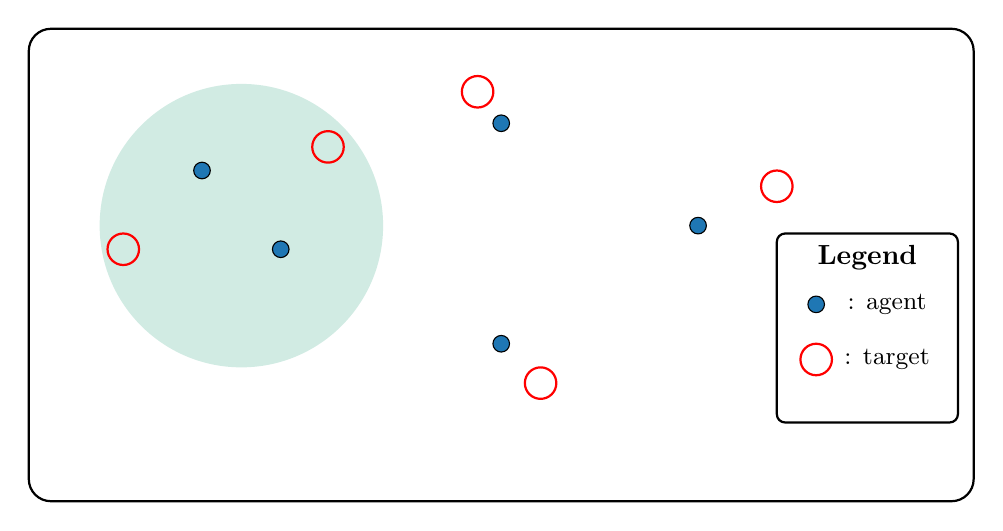
\begin{tikzpicture}
    \definecolor{agentblue}{RGB}{31,119,180}
    \definecolor{targetred}{RGB}{255,127,14}
    \definecolor{areagreen}{RGB}{140,205,185}

    % Rectangle border (environment)
    \draw[thick, rounded corners=8pt] (0,0) rectangle (12,6);

    % Green shaded area
    \fill[areagreen, opacity=0.4] (2.7,3.5) circle (1.8);

    % Agents (blue)
    \foreach \x/\y in {2.2/4.2, 3.2/3.2, 6/4.8, 6/2, 8.5/3.5} {
        \node[fill=agentblue, draw=black, circle, minimum size=6pt, inner sep=0pt] at (\x,\y) {};
    }

    % Targets (red circles)
    \foreach \x/\y in {1.2/3.2, 3.8/4.5, 5.7/5.2, 6.5/1.5, 9.5/4} {
        \draw[red, thick] (\x,\y) circle (0.2);
    }

    % Legend box
    \begin{scope}[shift={(9.5,1)}]
        \draw[thick, rounded corners=3pt] (0,0) rectangle (2.3,2.4);
        \node at (1.15,2.1) {\textbf{Legend}};
        \node[fill=agentblue, draw=black, circle, minimum size=6pt, inner sep=0pt] at (0.5,1.5) {};
        \node at (1.4,1.5) {\small : agent};
        \draw[red, thick] (0.5,0.8) circle (0.2);
        \node at (1.4,0.8) {\small : target};
    \end{scope}

    \end{tikzpicture}
    \caption{Illustration of localized coordination: agents (blue) only need to cooperate with nearby peers and local targets (red). Agents outside the green zone are operating in unrelated regions.}
    \label{fig:local-coordination}
\end{figure}

This insight suggests that \textbf{forcing full, global coordination at every step is both unnecessary and computationally inefficient}. In the scenario depicted, all five agents' Q-values are fed into the mixing network, and the full state of all agents conditions the hypernetworks, despite the fact that only two agents are operating in a tightly coupled sub-problem. This leads to redundant computation and a harder learning problem.

This inefficiency motivates the idea that \textbf{coordination can be made conditional and selective}, rather than global and rigid—a concept we explore in the next section.
\end{document}